\chapter{The Architecture of the SAFE Network}
\label{ch:architecture}

The internet is constantly growing and changing. Changes in technologies slowly permeate throughout the network as if by osmosis. Governmental policy can have a large impact on how people interact with the network, whether that be Turkey blocking Wikipedia or the US abandoning Net Neutrality. This area is where the SAFE Network starts to deviate greatly from the \textit{traditional} internet. The SAFE Network is a 'Autonomous Data Network'. To have access to the SAFE Network means to have access to all of it. A government cannot curate access data. This is made possible by the architecture of the SAFE Network.

\section{Vaults and Clients}

The SAFE Network is comprised of \textit{vaults}. A \textit{Vault} is a singular program/application that a user runs on their computer, whether that be a server hosted in a datacenter, a Raspberry Pi or a desktop computer. A \textit{vault} is given a set amount of storage by the user which it then uses to \textit{farm} data. For a given \textit{vault} to join the network, it must pass a 'Proof of Resource'. This initial test is used to validate that the \textit{vault} has enough bandwidth and CPU power to be able to adequately perform its job. Similar to how a real world farmer looks after their crop/animals, a \textit{farmer} (\textit{vault}) on the SAFE Network looks after data. Understanding that nomenclature is quite useful in understanding the function a \textit{farmer} (\textit{vault}) serves. Once \textit{vault} is successfully storing data it is rewarded with \textit{Safecoin}, which is a cryptocurrency hosted on the SAFE Network. Reading data from the network doesn't incur any cost, it is only when writing data that a user (\textit{client}) has to expend \textit{Safecoin}. A user doesn't need to run their own \textit{vault} to interact with the network, all users interact through the use of a \textit{client}. To help increase privacy, a \textit{client} connects to the network through an intermediary \textit{vault} called a \textit{proxy node}. This \textit{proxy node} orchestrates the writing and retrieval of data on behalf of the \textit{client}, hiding the \textit{clients} IP address from the rest of the network.

The only time a user interacts with their \textit{vault} is through configuration before startup. The most notable configuration being the allocation of storage for the \textit{vault}. Once \textit{vaults} start communicating with each other there is no intervention by humans. The network itself votes on and decides many factors. This includes everything from where data should be stored to how much value a \textit{Safecoin} has. This is the autonomy of the network, it does not accept governance by humans and \textit{vaults} cooperate for the good of the entire network.

\section{Immutable and Mutable Data}

Similar to BitTorrent data is broken down into chunks. Each ``chunk'' of data that is stored on the SAFE Network is at most 1MiB in size and has a unique 256-Bit Address. This allows every chunk of data to be uniquely identified and helps \textit{vaults} to decide who stores what data. Data stored on the SAFE Network can take one of two forms. It can either be \textit{Immutable Data} or \textit{Mutable Data}. A Mutable Data Structure (MD) is a \textit{key value} storage mechanism that allows for the storage of one thousand entries. An Immutable Data structure only stores a single ``value'', its address derived from the hash of the binary data it contains. An Immutable Data structure can itself only be 1MiB in size, but through the use of a \textit{Data Map} (Section \ref{subsec:self-encryption-data-map}) this limit can be subverted. As their names imply, Mutable Data can be freely mutated whereas Immutable Data cannot. It is this property of Immutable Data that eliminates duplication on the network. For example, if Bob uploads a picture to the network he is presented with the address of that file (possibly the address of a \textit{data-map}) and will have the relevant keys to access it. If Alice then uploads the exact same picture the data is not duplicated, she is simply presented with the same information that Bob was. If either Bob or Alice chooses to ``delete'' the picture, then they simply ``forget'' how to access that data. This means that if someone has access to a piece of data then that ability will never be revoked.

\subsection{Self Encryption and Data Maps}
\label{subsec:self-encryption-data-map}

\begin{figure}[h]
	\begin{center}
		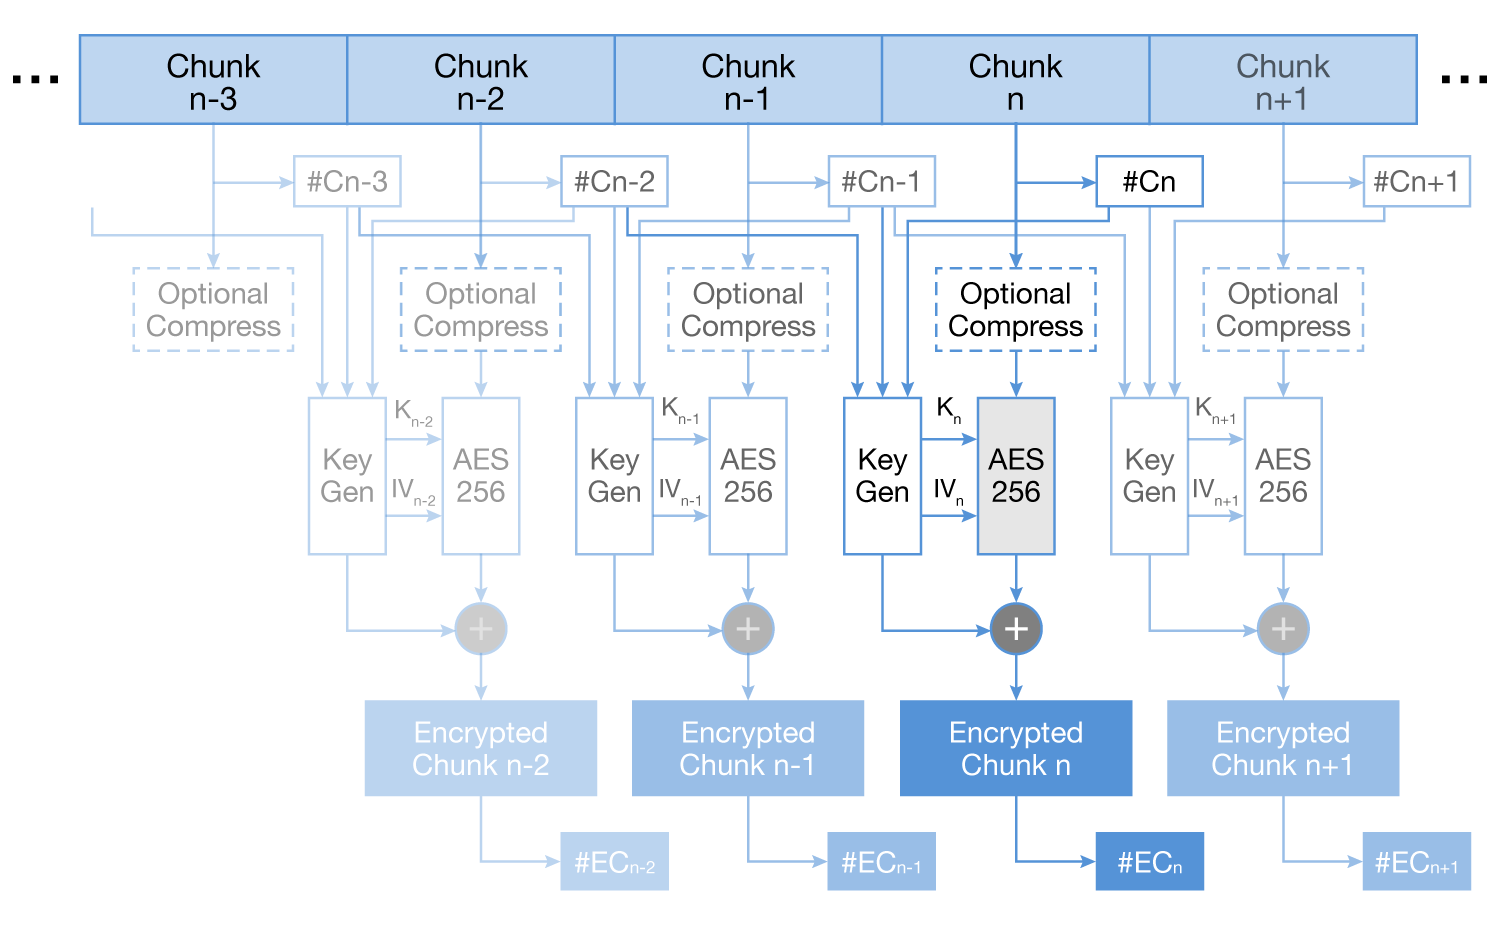
\includegraphics[width=\textwidth]{diagrams/self-encryption}
		\caption{The \textit{Self Encryption} process (sourced from https://safenetwork.wiki/en/Encrypt)}
		\label{fig:self-encryption}
	\end{center}
\end{figure}

Data that is stored on the SAFE Network goes through a process called \textit{Self Encryption}\cite{irvine2010self}. During \textit{self encryption} data is broken down into chunks of a specified size (The SAFE Network uses 1MiB chunks). To be able to reassemble and read the data a structure known as a \textit{Data Map} is created during the process. The \textit{Data Map} contains several pieces of information:

\begin{itemize}
	\item chunk\_num u32: Specifies how many chunks of data are within the Data Map
	\item hash Vec\textless u8\textgreater: Post-encryption hash of chunks
	\item pre\_hash Vec\textless u8\textgreater: Pre-encryption hash of chunks
	\item source\_size u64: The size of the original piece of data, before any encryption has taken place
\end{itemize}

The crucial structures of this \textit{Data Map} are the two vectors that store the pre-encryption and post-encryption hashes of chunks. The encrypted chunks of data are derived through the process of \textit{self-encryption}. What happens first is a piece of data is broken down into chunks and then hashed. The hash of the chunks is stored in the `pre\_hash Vec\textless u8\textgreater' of the \textit{Data Map}. This list is important as it defines the original piece of data before being encrypted. Each chunk then goes through an encryption process using AES 256. The key used for each chunk is the pre-encryption hash of one of the other chunks. The chunks then go through another step that further obfuscates the data. This step involves XOR'ing the data with the pre encryption hash of other chunks. A final hash is then taken of each chunk and stored in the `hash Vec\textless u8\textgreater' of the \textit{Data Map}. You can see the process of \textit{self encryption} in Figure \ref{fig:self-encryption}.

\textit{Self Encryption} is a generic process, there is nothing about it that specifically ties it to the SAFE Network. \textit{Self Encryption} is used to obfuscate data for storage, It is only with access to the \textit{Data Map} that you can make sense of the data. It is through this obfuscation process that means \textit{vaults} cannot distinguish what the chunks they are storing actually contain. It is just ``garbage'' data to them. This means chunks can be freely distributed across the network with the assurance that only the person with access to the \textit{Data Map} can read the original data.

\subsection{Address Collision}
\label{subsec:address-collision}

The SAFE Network stores chunks based on their 256-Bit address. Although the probabilities are unfathomably small, collisions in the post encryption hash of chunks from \textit{self-encryption} is possible. The hash algorithm used currently is \textit{SHA3-256}\cite{dworkin2015sha} which was first published in 2015. \textit{SHA3-256} is an incredibly ``safe'' hashing algorithm to use, papers like \citetitle{amy2016estimating}\cite{amy2016estimating} do propose methods on how to ``break'' the algorithm but their findings indicate that even with Quantum computers an attack would be practically unfeasible. The question as to why use \textit{SHA3-256} when stronger algorithms exist within the same family is however curious. NIST themselves currently recommend\cite{hash-reccomend} that for generic hashing applications \textit{SHA3-512} is the minimum algorithm that should be used. This brings into question why Maidsafe have chosen a less secure algorithm. If the choice came down to performance then this is an oversight that could hurt them greatly in the long run. Moore's law\cite{schaller1997moore}, however debatable that it still applies, dictates that as time passes computers become more and more capable. If the SAFE Network truly wants to exist for a long period of time, choosing \textit{SHA3-256} as the algorithm the entire network is based upon seams like a naive approach. The suggestion to use the strongest algorithm that exists today is thus highly encouraged, a switch to \textit{SHA3-512} seams like a logical step.

\subsection{True Immutability of Data}
\label{subsec:immutability-of-data}

Once data has been written to the network, it can never be changed. The chunks of data that are the result of \textit{self encryption} will be stored by the network indefinitely. This means that to ``delete'' data more accurately means to ``forget how to access it''. The implication of this is that once data is uploaded, access to the \textit{Data Map} is the only think that stands between being able to access the data and it being lost forever. This has big implications and benefits to some use cases, think archiving books or genealogical records.

\subsection{Disjoint Sections}

The unique address of every 1MiB chunk of data is used to determine what \textit{vaults} are responsible for storing it. Maidsafe's innovation was in the creation of what are called \textit{Disjoint Sections}. These \textit{sections} are groups of \textit{vaults} that are responsible for a certain range of the 256-Bit XOR Address Space. By default, the network requires a minimum number of \textit{vaults} to sustain the network. At the time of writing this is eight \textit{vaults}. These eight \textit{vaults} form a complete \textit{section} and are responsible for the storage of the entire 256-Bit address range. As more \textit{vaults} join the network, this \textit{section} will grow in size and then eventually split into two new \textit{sections}. There are numerous requirements that have to be met before a \textit{section split} is allowed.

% Insert equation for section split

\begin{figure}
	\begin{center}
		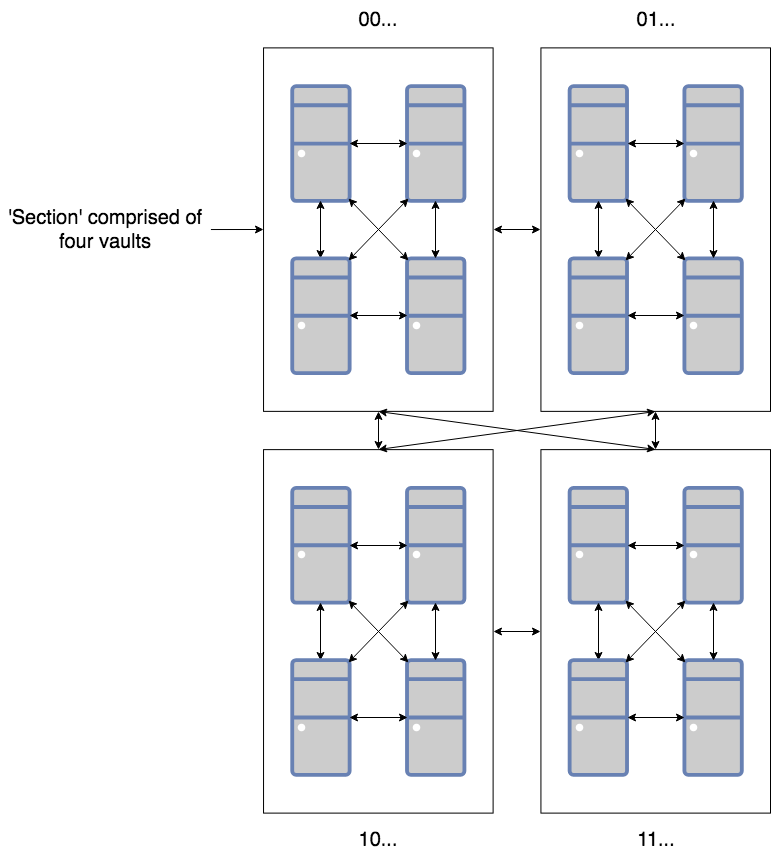
\includegraphics[scale=0.3]{diagrams/safe-network-sections}
		\caption{Four sections of a SAFE Network. You can see the address range each section is responsible for.}
		\label{fig:safe-sections}
	\end{center}
\end{figure}

After a split, \textit{sections} are then responsible for half of the 256-Bit address range that they were before. As more and more complete \textit{groups} of ~8 \textit{vaults} join the network, it continues to split and each \textit{section} is therefore responsible for the curation of less and less data. An important thing to note is that the SAFE Network doesn't assign 256-Bit addresses based on proximity, in a given section two \textit{vaults} could be very close together in 256-Bit XOR space but be located on different continents. This property helps the integrity of the network by ensuring \textit{vaults} in a given section are not located close to each other. Otherwise the network could be open to simple attacks. For example, start 8 \textit{vaults} on a single computer to form a \textit{section} then suddenly switch them all off which could cause data loss. If a significant number of \textit{vaults} leave the network then \textit{sections} have the ability to join with other \textit{sections} to ensure the stability of data is maintained. In Figure \ref{fig:safe-sections} you can see four \textit{sections} comprised of four \textit{vaults} each, you can see the address range that each \textit{section} is responsible for. In the diagram four \textit{vaults} make a \textit{section} instead of the traditional eight, this is just to make the diagram easier to process.

\subsection{Proof of Resource}
\label{subsec:proof-of-resource}

The \textit{proof of resource} (PoR) test is used to valid the effectiveness of a \textit{vaults} ability to store and serve data and is the value proposition of \textit{Safecoin}. The PoR is used to validate \textit{vaults} joining the network but also during other network events. Such an event is proving to its \textit{section} that it is indeed storing the data it says it is.

\subsection{Personas}

\textit{Vaults} can be characterised as having different ``Personas''. One such \textit{persona} is the \textit{Data Manager}. A \textit{Data Manager} is responsible for the storage of chunks within a a\\textit{section}. Their job is vital to the stability of the network. When data is stored on the network, it is actually replicated across multiple \textit{Data Managers}. At all times the network aims to keep a minimum number of copies of a chunk of data, if a chunk goes missing this chunk is replicated to another \textit{Data Manager} to ensure that data is stored redundantly. Hence within a given section, there will be several vaults storing identical chunks of data. Each having full knowledge of the chunks of data that the other \textit{Data Manager} hold. This scheme means that no \textit{vault} will ever hold the single copy of a chunk of data, meaning that data is stored redundantly across the network.

Another important \textit{persona} is that of the \textit{Client Manager}. A \textit{Client Manager} is responsible for storing the account data for clients that fall within its address space. When you create an account on the SAFE Network the data is stored on the network just like any other piece of data. It has a given 256-Bit Address and contains information like: how much \textit{Safecoin} an account has, the number of chunks of data that has been uploaded, etc. As an account is a 256-Bit address it will fall within the domain of a particular section, the \textit{Client Managers} in that \textit{section} will then store the relevant data.

\subsection{Accounts}

Accounts on the SAFE Network are not inherently special in that they are stored along with other pieces of data on the network. There is no centralised body or organisation that is needed to grant access to the network. An account on the SAFE Network is derived from two parts, an \textit{Account Secret} and a \textit{Account Password}. The \textit{Account Secret} identifies where the account is stored then the \textit{Account Password} is used to encrypt and decrypt the information. From these two components a client can gain access to a piece of data that represents their account. This data structure leads to all the data needed for the account:

\begin{itemize}
	\item The Safecoin balance of the account
	\item Address(es) of \textit{Data Maps} that the account has decryption keys for
	\item Decryption keys for the aforementioned \textit{Data Maps}
	\item Other account information
\end{itemize}
	
A single login secures all of their data behind multiple layers of encryption meaning they just need one set of credentials to access the network and their data. An important caveat in this is that once credentials are lost, the account can never be accessed again. This is not a real problem for ``professional'' users as most make use of password managers and other such tools. At some point though even the most ``pro'' user could lose track of a password and with that their data is gone. There is no chance of recovery. This could involve losing irreplaceable data which can be heart-breaking for individuals and bankruptcy causing for companies. Thus keeping credentials safe is extremely important. This could be a prohibiting factor to a lot of users however, some may just not want to take the risk.

\section{Crust and Encryption}

\textit{Crust} is the secure routing layer designed and built by Maidsafe to provide the secure communications backbone of the SAFE Network. \textit{Crust} allows for reliable P2P connections and provides encryption for all traffic. Several Transmission Protocols can be used, falling back to UDP from TCP (for example) if required. Encryption at this level means that Data on the network is always encrypted, data is only decrypted client side and whenever it is not on a clients computer it is fully encrypted.

Encryption is a very important aspect of the SAFE Network. Whenever data is stored on the network, it is encrypted. Data on the network exists as discrete 1Mb chunks, each with its own 256-Bit Address. When a file is uploaded to the network, it undergoes a process known as \textit{self encryption}. As mentioned in Section \ref{subsec:self-encryption}, \textit{Self Encryption} is a technique that is used to break data down into 1MiB chunks and also to encrypt each chunk. These are the chunks that are ultimatly stored by \textit{vaults}. You can choose to have data ``unencrypted'' or what Maidsafe calls ``Plain'', what this means is that any user that knows the address of the data (and the type-tag) can retrieve and read the data. The special thing about this is that the data is still fully encrypted on the network through \textit{self encryption}, a \textit{vault} owner cannot decipher what the chunk of data holds. When anyone goes to access this data though, it is reassembled and you can read it. The two other types of encryption supported are Symmetric and Asymmetric. Through different key exchange mechanisms you can use these forms of encryption to build interesting applications.

\begin{figure}
	\begin{center}
		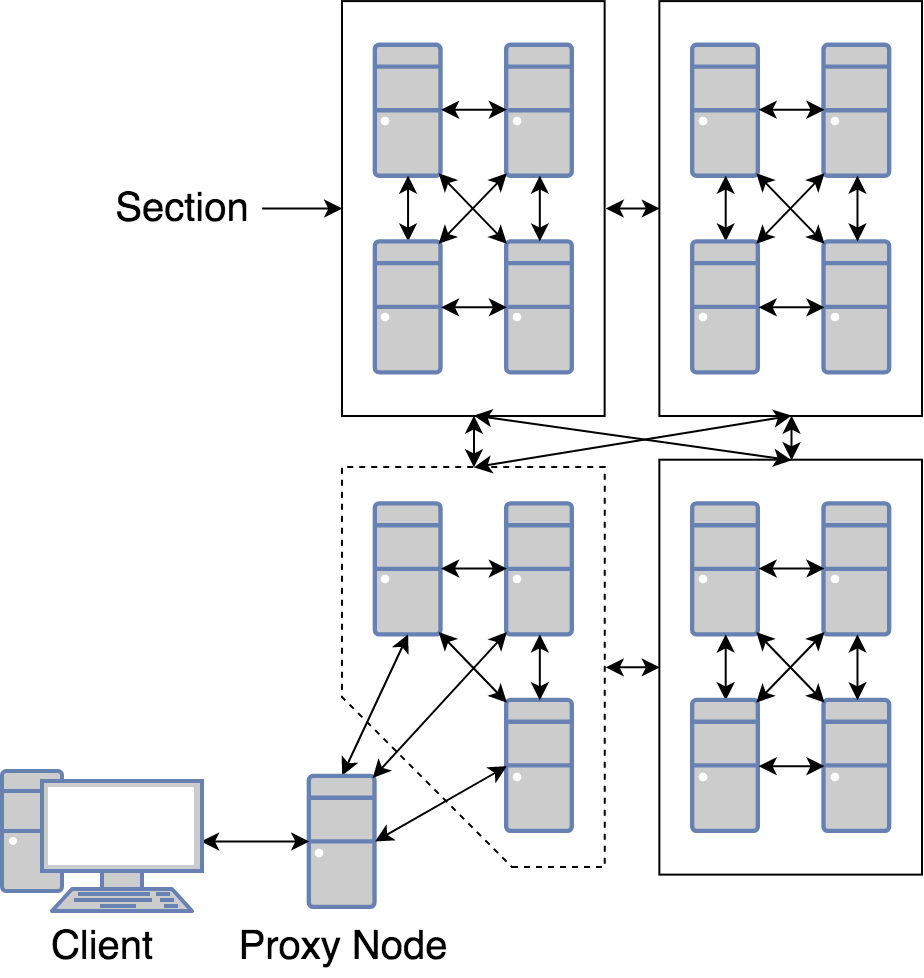
\includegraphics[scale=0.3]{diagrams/safe-network-connection}
		\caption{A client connecting to the SAFE Network through a Proxy Node}
		\label{fig:proxy-connection}
	\end{center}
\end{figure}

When a client connects to the network they do so through the use of a \textit{Proxy Node}. A \textit{Proxy Node} is a \textit{vault} that is used to liaise between a client and the network at large. The \textit{Proxy Node} is used to hide the clients IP address from the rest of the network. Beyond the proxy and deeper into the network all \textit{vaults} know is the XOR Address of the account being used and its Public Key. Hence by using a \textit{Proxy Node}, the real world identity of the client is well hidden from the rest of the network. This means that a given \textit{vault} cannot detect that the data it is sending is going to a certain geographical location. In Figure \ref{fig:proxy-connection} you can see the topology of how a client connects to the SAFE Network.

\section{Safecoin and Farming}

Safecoin\cite{lambert2015safecoin} is the cryptocurrency of the SAFE Network, it is earned by \textit{farmers} and spent by writing data to the network. The expectation is that as the cost of CPU/Storage falls with time, the value of the Safecoin will increase. Value in this context is how much data each coin facilitates the storage of.

When a user creates an account on the network, they are given a \textit{Safecoin} wallet. This wallet can be used to securely store the \textit{Safecoin} that belongs to the account. Akin to \textit{Bitcoin}, \textit{Safecoin} is a cryptocurrency. It can be sent between users in a permission-less manner. \textit{Safecoin} can be sourced in a number of ways including through \textit{farming} and by simply purchasing them with another currency. The ultimate purpose of \textit{Safecoin} is to incentivise people to run \textit{vaults}. Running a \textit{vault} is costly, so the reward of \textit{Safecoin} is used to incentive the participation of nodes in the network.

\textit{Farming} is the action of \textit{vaults} to store, maintain and serve data to clients. When a client requests a chunk of data, the \textit{vault} that successfully returns that piece of data will be given the opportunity to earn \textit{Safecoin}. The probability of being awarded this attempt to earn \textit{Safecoin} is determined by the \textit{farming rate} of the network at that specific moment in time. The \textit{farming rate} is used to balance supply and demand of data on the network. The SAFE Network tries at all times to keep a minimum amount of network capacity free, this is around \%30. When free space starts to fall below this threshold then the \textit{farming rate} will increase, meaning \textit{vaults} have the opportunity to earn more \textit{safecoin}. This works in the opposite direction too. If the network capacity grows so that there is an overabundance of free space then the \textit{farming rate} will decrease meaning \textit{vaults} earn less money. This constantly varying \textit{farming rate} is hence used to balance network resources and de-incentivise users adding \textit{vaults} with very high capacity to the network (if it is not needed). It encourages more \textit{farmers} when the network is running low on capacity (compared to demand) and discourages them when resources are overabundant.

The economics of \textit{Safecoin} are a subject that is out-with the scope of this paper. In short, its utility on the SAFE Network is not tied to whatever its `exchange price' is. Overtime, the storage `buying power' of each \textit{Safecoin} should increase as computing power and storage becomes cheaper. \textit{Safecoin} is in its infancy and indeed has not yet been implemented. This means it is subject to changes (however this is unlikely) from what has been described above. There are proposals upon how to build the \textit{Safecoin} support structure into the SAFE Network but as it has not been implemented yet I will avoid going discussing it in this paper.

\section{Quorum and the Datachain}

As the network acts as an autonomous entity there has to be some method for a given \textit{vault} to reach consensus with other \textit{vaults}. This problem is what Cryptocurrencies aim to solve through processes such as mining. \textit{Mining} is essentially the network reaching consensus upon what has happened (in this case, financial transactions). In the case of \textit{Bitcoin}, every time a block is \textit{mined} it is cryptographically linked to the block that came before it. As this \textit{Blockchain} grows in size, the consensus on past transactions grows and grows. For \textit{Bitcoin} and similar \textit{cryptocurrencies}, to be able to undo a transaction/block you would need to have control of over \%50 of the networks \textit{mining} power. The SAFE Network needs a similar mechanism on how to reach consensus. Analogous to a \textit{Blockchain}, the SAFE Network has a \textit{Datachain}. 

The Datachain is used to help insure the integrity of the network and can be used to help rebuild it in the case of a catastrophic failure. For any action on the network to be valid, whether this be the storing/mutation of data or a \textit{vault} joining a \textit{section}, there has to be a corresponding \textit{group signature}. This \textit{group signature} is stored in the \textit{Datachain} that all \textit{vaults} in a \textit{section} have. In order for an action to be considered valid, a \textit{section} has to reach a quorum. For a network where the minimum \textit{section} size is eight, a quorum would be five out of the eight vaults voting in agreement. This means that in a given \textit{section}, several \textit{vaults} could be acting as ``bad parties'' but network integrity wouldn't be lost. XOR Distance also comes into play in this process. The closer two \textit{sections} are in 256-Bit XOR Address Space the more they know about the data the other \textit{section} is storing. They will have access to the portion of the \textit{Datachain} that is used by that \textit{section} that is used to record data writes and mutation. This way a given \textit{section} can help to verify that a neighbour is acting as a good party in the network and that data being stored there has not been tampered with. The further away in 256-Bit Address Space two \textit{sections} are then the less they know about each other. This means that as the number of \textit{sections} increases, the influence a given a \textit{section} has over the network decreases. Eventually resulting in no \textit{section} in the network having an overview of the entire network.

A protection mechanism exists in the retrieving of data for when a vault tampers with data after it has been recored in the \textit{Datachain}. When a client requests a given piece of data, a single \textit{vault} is chosen to return that chunk of data. Alongside the data that is returned, a minimum number of acknowledgements from other \textit{vaults} in the section must be returned too. This way, a client can then verify the data they receive against the acknowledgements from the other vaults in order to ensure that the data is valid.

The development of the \textit{Datachain} is still very active, at the time of writing I have tried my best to summarise the current proposals. Thus the \textit{Datachain} is still very much subject to rapid range.

\subsection{Node Age and Churn}

A crucial part of the integrity of the \textit{Datachain} is \textit{node ageing}. For a \textit{vault} to \textit{vote} on network activity (this is the signatures that form the \textit{group signature}) it has to have proved itself a reliable node. A \textit{vault} cannot just join the network and start voting in network decisions. When a new \textit{vault} announces itself to the network, it is issued with the \textit{Proof of Resource} that was discussed in Section \ref{subsec:proof-of-resource}. If it passes then as long as the assigned \textit{section} reaches a quorum the \textit{vault} will join that \textit{section}, recording its membership in the \textit{Datachain}. This node is very ``young'' in the eyes of the network and as such is not trusted. It is not allowed to vote in group actions and is responsible only for the storage and transmit of data. A very interesting aspect of the SAFE Network is the concept of \textit{churn}. 

\textit{Churn} is used to constantly 'rotate' vaults round different \textit{sections} on the network. This means that in a given time frame, a \textit{vault} will not be responsible for the same 256-Bit address range. This important feature helps to ensure that it is very difficult to track down where data is stored in order to erase it or corrupt it. During churn, young \textit{vaults} with a lower \textit{node age} will be chosen more frequently than older \textit{vaults}. The \textit{vaults} chosen are assigned to new \textit{sections} to which it must give another \textit{proof of resource} to be allowed to join. If the new \textit{section} reaches quorum then the \textit{vault} joins and its \textit{node age} is incremented. Thus, trust must be earned by acting as a good party in the network over time. Only when a \textit{vault} reaches a certain \textit{node age} does it become an \textit{elder}. An \textit{elder} is a node which has the highest possible \textit{node age}, meaning it has has proven itself to be a reliable party over the course of time. When a \textit{vault} is an \textit{elder}, it gains the voting rights that eventually lead to the construction and maintenance of the \textit{Datachain}. If a\textit{vault} acts out of order then its \textit{node age} can be decremented or eliminated entirely. Trust must be earned.

\textit{Node ageing} and \textit{churn} are hence essential security features of the network and make it very difficult for an attacker to have any choice in the \textit{section} of the network they wish to attack.
